\documentclass[./standalone.tex]{subfiles}
%\documentclass[../../../CR/pac.tex]{subfiles}

\begin{document}

% --------------------- %
%          PART         %
% --------------------- %
\part{Manuel du joueur}

% Section:
\section{Qu'est-ce que Silent In Space?}
Silent In Space (abrégé : “SIS”) est un jeu Point \& Click s'inspirant des Monkey Island. Dans ce jeu, vous vous réveillez dans un vaisseau alien et avez pour but de vous en échapper. Faites-vous des alliés ou des ennemis sur votre chemin et découvrez pourquoi vous êtes ici! 

% Section:
\section{Lancer le jeu}
Le jeu se lance dans un IDE de type Intellij IDEA ou NetBeans. Il nécessite \color{red}Java 15 \color{black} et \color{red}JavaFX 16\color{black}.\\ 

Si vous choisissez de le lancer dans un IDE Intellij vous devez:
\begin{enumerate}
	\item Aller dans la structure du projet (File > Project Structure)
	\item Ajouter la librairie - ie. le dossier lib/ - de  JavaFX (Libraries > + > Java > lib/)
	\item Aller dans les paramètres d'exécution (Run > Edit Configurations)
	\item Cliquer sur l'application "Main" et ajouter dans le champ \textit{VM options} : $--$module-path "../librairies/javafx/lib" $--$add-modules=javafx.controls,javafx.fxml
\end{enumerate}

\begin{center}
	\begin{figure}[h!]
	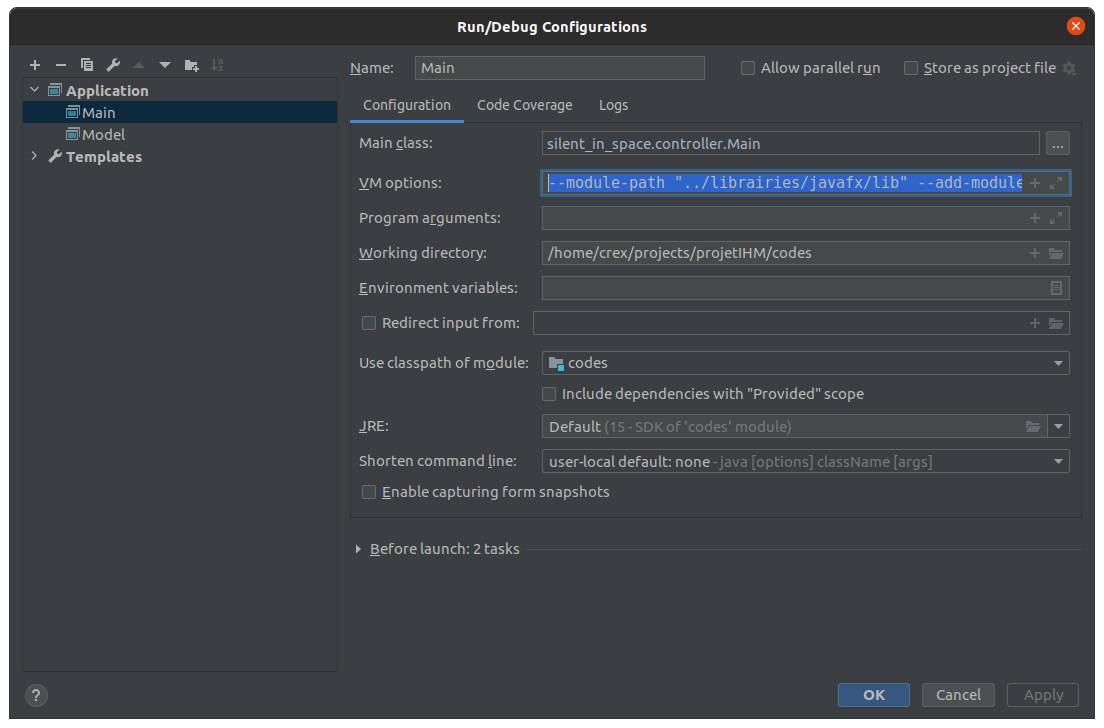
\includegraphics[scale=0.4]{images/vm_options.png}
	\caption{Configuration du Runner d'Intellij pour JavaFx}
	\end{figure}
\end{center}

\newpage

% Subsection:
\section{Les contrôles du jeu}

\begin{tabular}{| m{40em} |}
\hline
	\begin{center}
	   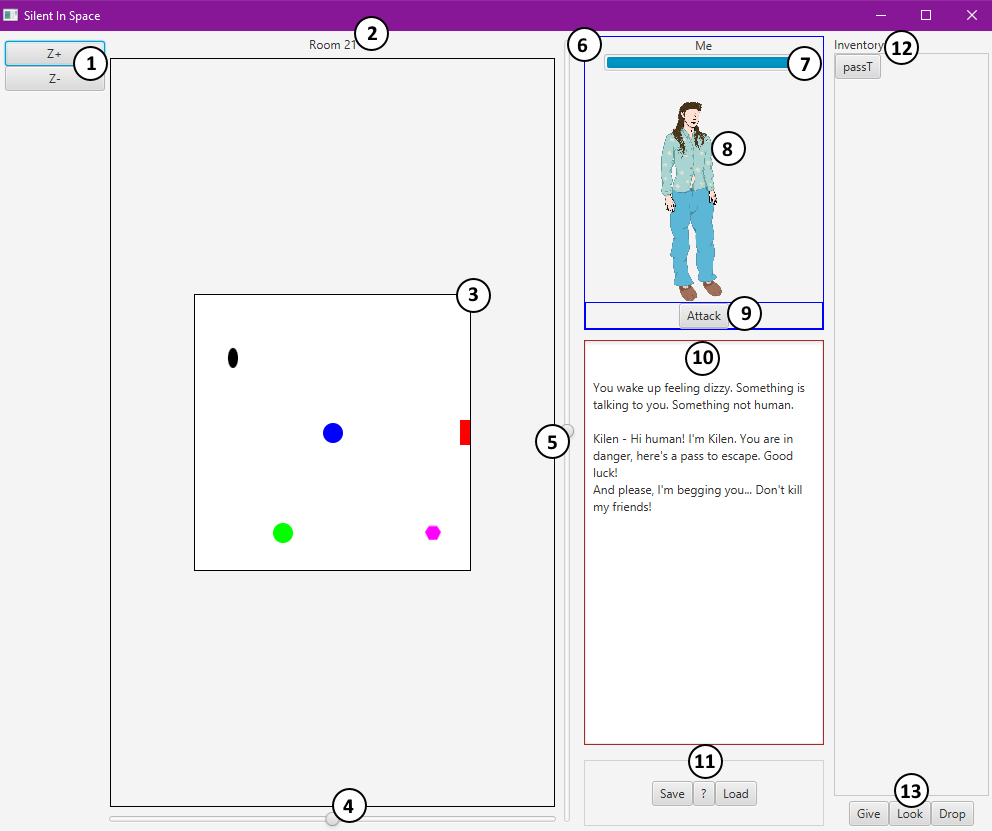
\includegraphics[scale=0.4]{images/UI.png}
	\end{center}\\
\hline
	\begin{enumerate}
		\item Fonctions de Zoom sur la carte
		\item Numéro de la pièce actuelle
		\item Panneau de la Carte de Jeu. C’est ici qu’évoluera la vue des pièces et leurs contenus
		
		\item Slider permettant de déplacer la vue sur l'axe horizontal
		\item Slider permettant de déplacer la vue sur l'axe vertical
		\item Panneau des personnages
		
		\item Barre de vie du personnage sélectionné
		\item Illustration du personnage sélectionné
		\item Bouton d’Attaque
		
		\item Panneau de Dialogues. C’est ici que sera affiché le texte en jeu
		\item Boutons de Sauvegarde et de Chargement. Appuyer sur “?” fera apparaître le manuel du jeu.
		\item Panneau de l’Inventaire. Chaque nouvel item ramassé par le joueur apparaît ici.
		
		\item Boutons relatifs à l’Inventaire. “Give” donne un item à un personnage, “Look” donne une description d’un item, et “Drop” lâche un item sélectionné au sol.
	\end{enumerate}\\
\hline
\end{tabular}
\newpage


\paragraph{Carte de Jeu\\}
    La carte du jeu \textbf{(3)} affiche le contenu de chaque pièce. Un clic droit sur n’importe quel élément (item, personnage, porte…) en affichera la description dans le panneau des dialogues \textbf{(11)}.
\par Utiliser les sliders \textbf{(4 et 5}) permet de déplacer la pièce et cliquer sur les boutons Z+ et Z- \textbf{(1)} permettent de zoomer et dézoomer.

\paragraph{Interactions avec les portes\\}
    Les portes sont symbolisées par un rectangle noir ou rouge placé contre un mur. Leurs localisations dépendent de l’emplacement de la pièce à laquelle cette porte conduit. Si la porte est à droite sur la carte du jeu \textbf{(3)}, la pièce à laquelle elle mène se trouve à droite. 
\par Les portes noires sont déverrouillées et les portes rouges sont verrouillées. Cliquer sur une porte déverrouillée permet de passer à la pièce à laquelle elle mène. Une porte verrouillée ne peut pas être empruntée si elle n’a pas été déverrouillée au préalable avec un pass ou un ordinateur.
        
\paragraph{Interactions avec les objets\\}
    Il existe deux types d’objets avec lesquels il est possible d’interagir :
    \begin{itemize}
    	\item ceux représentés par un hexagone rose (stations) 
\includegraphics[scale=1]{images/hexagone.png}
    	\item ceux représentés par un ovale noir (items)
\includegraphics[scale=1]{images/ellipse.png}
    \end{itemize}
            
\paragraph{Stations\\}
    Les stations sont des objets que le joueur ne peut pas ramasser. Faire un clic gauche dessus permet de les utiliser suivant la fonction qui leur a été assignée préalablement (obtenir une information en lisant un panneau, se soigner, etc.).
            
\paragraph{Items\\}
	Les items peuvent être ramassés par le joueur avec un simple clic gauche. Un item ramassé est ensuite affiché dans l’inventaire, dans la partie droite de l’écran \textbf{(12)}.
        
\paragraph{Interactions avec un personnage\\}
Vous pouvez sélectionner un personnage en faisant un clic gauche sur son icône sur la carte \textbf{(3)}. Lorsque vous sélectionnez un personnage, son portrait apparaît dans le panneau des personnages \textbf{(6)} et vous lui parlez. Une fois cela fait, vous pouvez l’attaquer (bouton d’Attaque, \textbf{9}) ou lui donner un objet (bouton Give, \textbf{13}).
        
\paragraph{Interactions avec l’Inventaire\\}
    L’inventaire affiche tous les objets obtenus par le joueur. Avec les boutons “Give”, “Look” et “Drop” \textbf{(13)}, le joueur peut manipuler ceux-ci de plusieurs manières.

\paragraph{Utiliser un item sur un objet\\}
	Pour cela il faut cliquer sur l’item dans l’inventaire \textbf{(12)}, puis cliquer sur l’objet ciblé dans la vue \textbf{(3)}. Cela permet par exemple de déverrouiller une porte.
        
\paragraph{Donner un item à un personnage\\}
    Il faut sélectionner le personnage à qui donner l’objet, sélectionner l’objet puis cliquer sur le bouton “Give”.
        
\paragraph{Boutons Look et Drop\\}
    Pour utiliser ces boutons, il suffit de sélectionner l’item dans l’inventaire \textbf{(12)} puis de cliquer sur le bouton voulu.
\newpage
    
% Subsection:
\section{Carte du jeu et Solution}
\begin{center}
	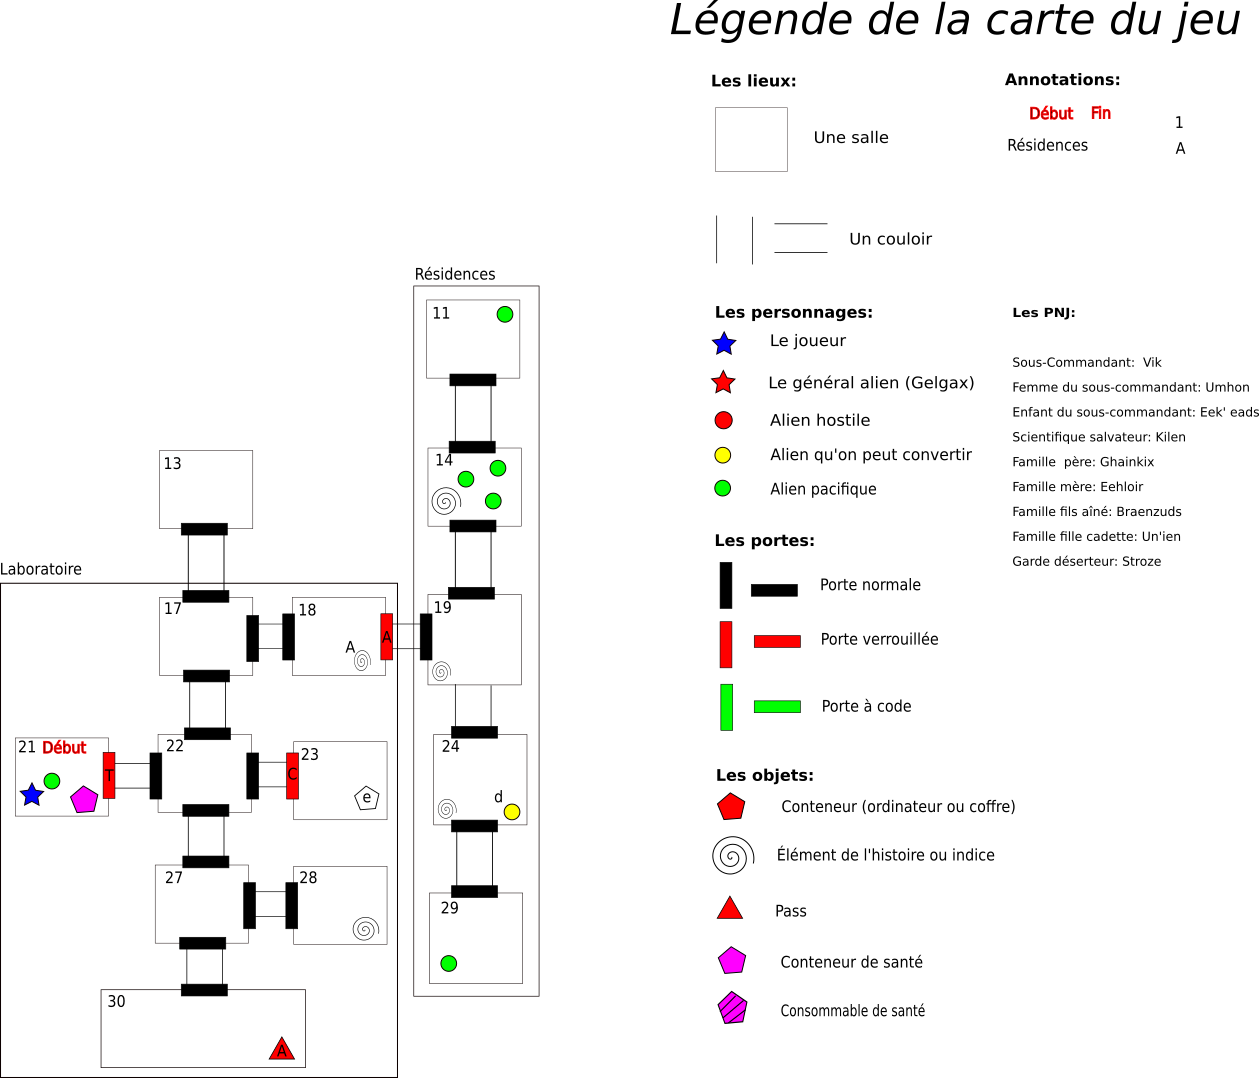
\includegraphics[scale=0.5]{images/v4.png}
\end{center}

Commencez par utiliser le passT sur la porte T et sortez de la pièce de départ. Rendez-vous en salle 30, puis récupérez le pass A. Vous pouvez maintenant vous rendre en pièce 18, et débloquer l’aile résidentielle du vaisseau.\\
 
Pour finir le jeu, vous aurez besoin de récupérer le code de l’ordinateur du capitaine. Il se trouve que la personne qui le possède n’est autre qu’Umhon, en salle 24. Cependant elle ne vous l’échangera uniquement que contre une preuve des expériences faites sur les humains sur le vaisseau. Vous avez alors deux option pour l’obtenir :
\begin{itemize}
	\item Tuer Umhon, et récupérer le code sur son cadavre
	\item Aller en salle 23. La porte se fermera automatiquement derrière vous. Utilisez l’ordinateur pour la débloquer, ainsi que pour imprimer le document “doctorLog”. Retournez voir Umhon et donnez-lui ce document.\\
\end{itemize}

Vous devez ensuite vous rendre dans la salle 13 pour déclencher la fin du jeu.


% Subsection:
\section{Recommandations pour le confort du jeu}
Une carte du jeu sans les solutions vous est fournie. Vous pouvez partager votre écran en deux parties comme dans l’image ci-dessous. Ainsi il sera plus facile de vous orienter dans le vaisseau spatial et de compléter les objectifs !

\begin{center}
	\begin{figure}[h!]
	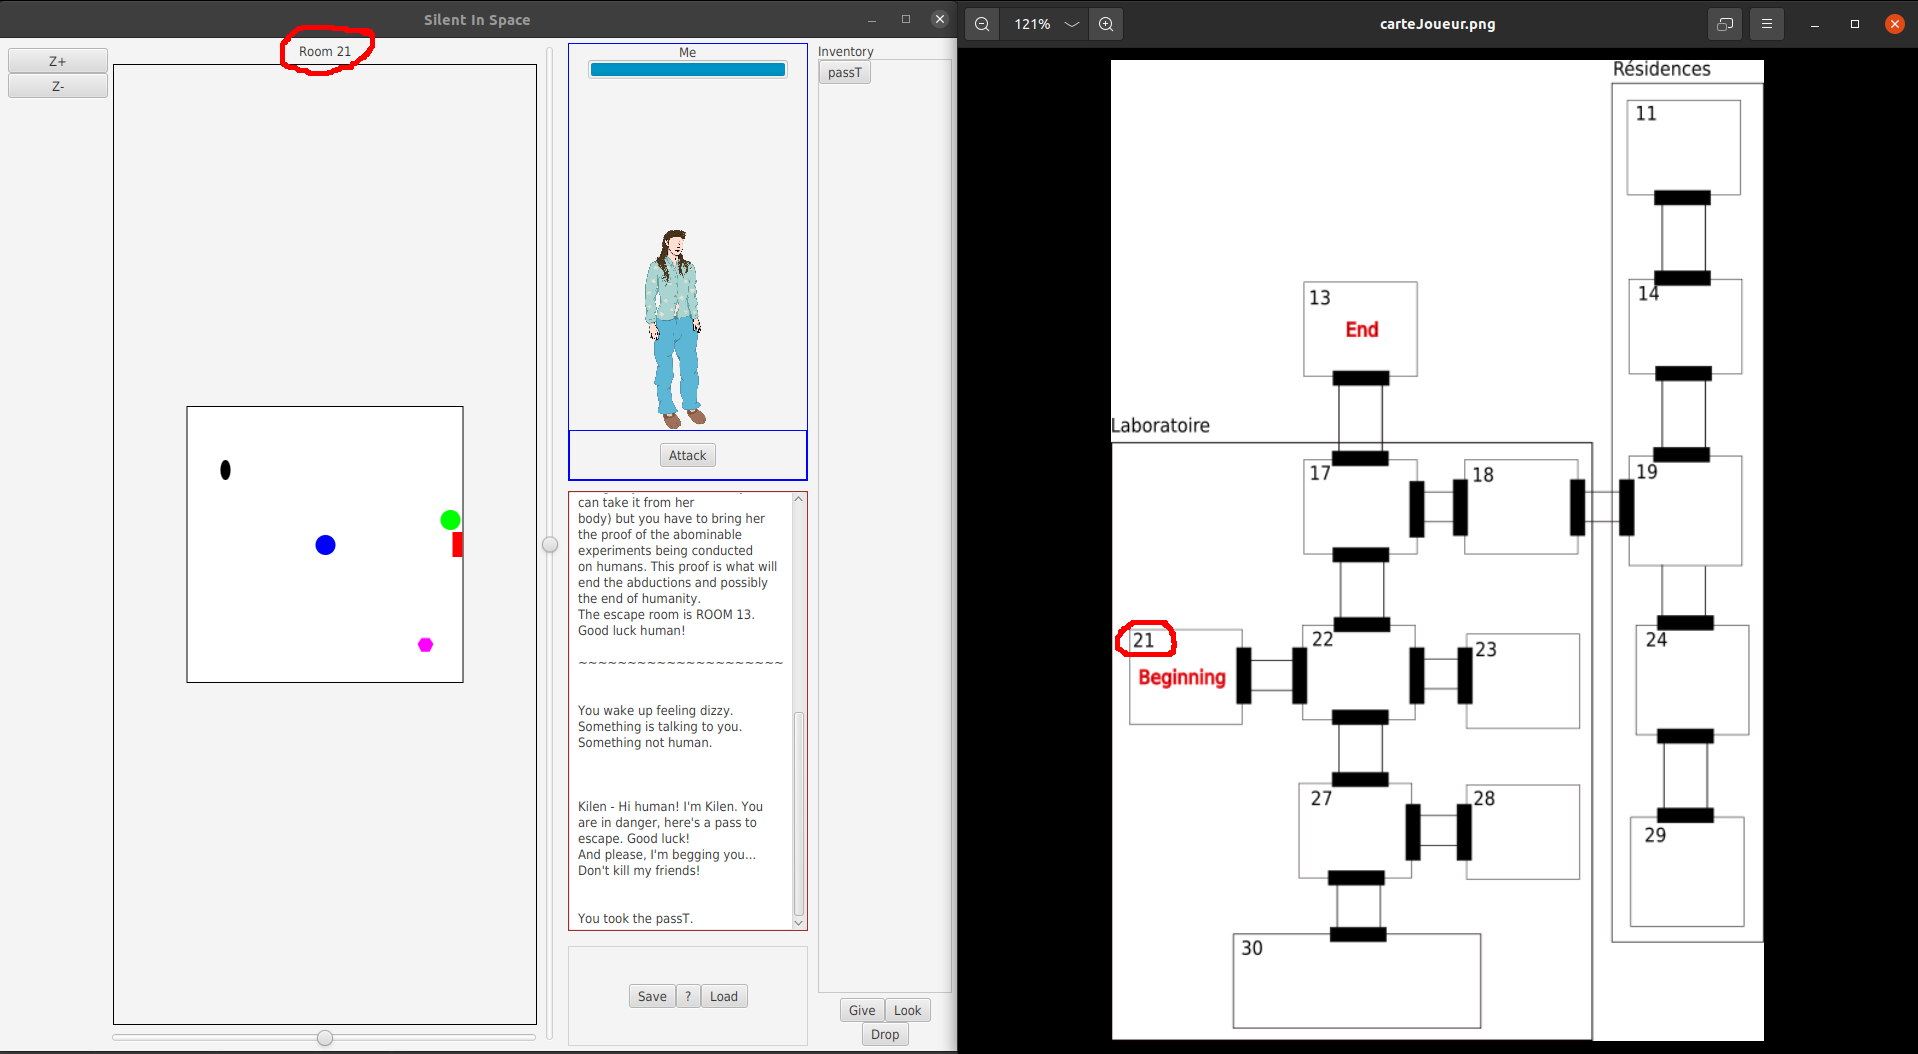
\includegraphics[scale=0.24]{images/conseils_utilisation.png}
	\caption{Entourés en rouge sont les indicateurs qui vous aideront à vous orienter à tout moment dans le jeu}
	\end{figure}
\end{center}


\newpage
% --------------------- %
%          PART         %
% --------------------- %
\part{Manuel du développeur}

% Section:
\section{Diagramme de classe du modèle}

Bien que le modèle ne soit pas le coeur de ce projet nous pensons que présenter ce-dernier vous permettra de mieux comprendre les quelques adaptations que nous avons dû y apporter pour l'application actuelle.\\

Ce diagramme de classe représente la hiérarchie des classes du modèle dans son état final lors de la remise du semestre dernier. Il ne s'agit pas de la hiérarchie actuelle! Bien que peu de choses ont changé.\\

\begin{flushleft}
	\begin{figure}[h!]
	\advance\leftskip-2.2cm
	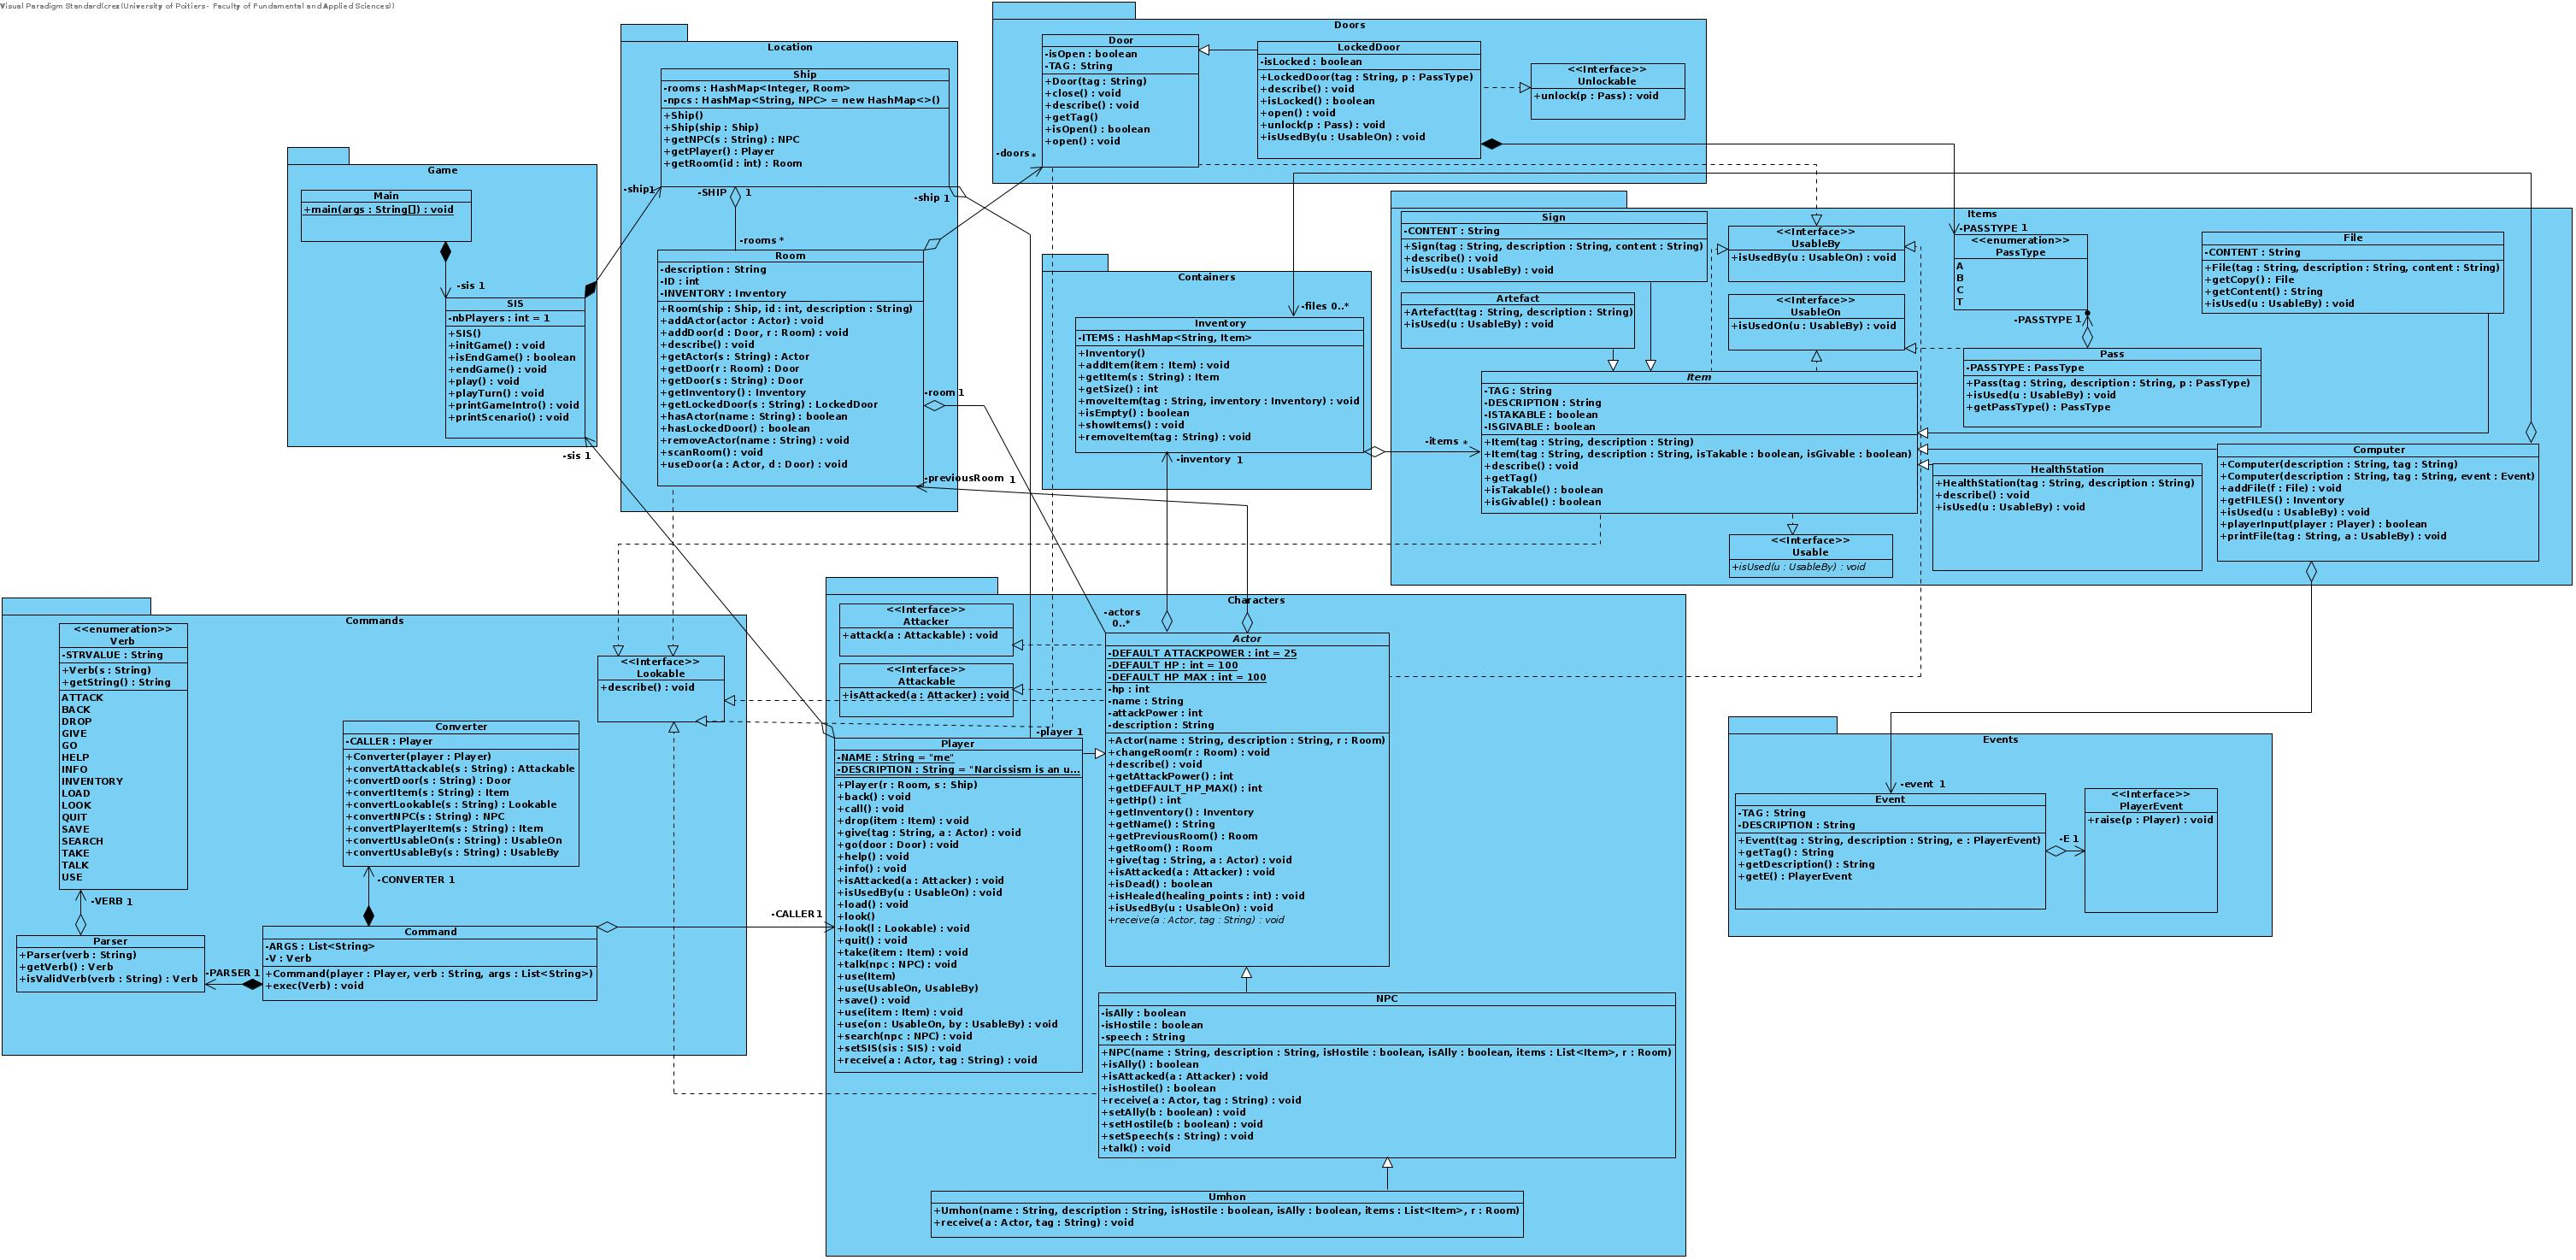
\includegraphics[scale=0.19]{images/SIS.jpg}
	\caption{Le diagramme en taille originale est fournie dans le dossier docs/ de l'archive du projet}
	\end{figure}
\end{flushleft}

Ainsi, nous avons rajouté un nouveau package: le package \textit{Utils}, qui n'est pas représenté sur ce schéma et dont l'unique classe \textit{Scalar2D} est composé dans les classes \textit{Actor}, \textit{Item} et \textit{Door}. Cette classe sert à indiquer des positions proportionnelles (aucune unité de mesure ne leurs sont associées) des objets/acteurs/portes les uns par rapport aux autres.\\

Une interface et une classe abstraite statique ont été ajoutée au package \textit{Game}: l'interface \textit{MessageListener} et la classe abstraite statique \textit{Message}.\\

La classe abstraite statique \textit{Message} a été conçue en nous inspirant de la fonction \textit{System.out.print()}: accessible partout et non instantiable. L'interface \textit{MessageListener} est inspirée des écouteurs de javaFX. Nous avons ainsi notre propre système d'écoute des messages du modèle: s'y abonnent les classes qui lui souhaitent, peu importe si elles sont dans un modèle ou une vue ou encore ce qu'elles font de ces messages.

\newpage

% Section:
\section{Structuration de l'application}

Voici un schéma expliquant le fonctionnement global de notre application:

\begin{center}
	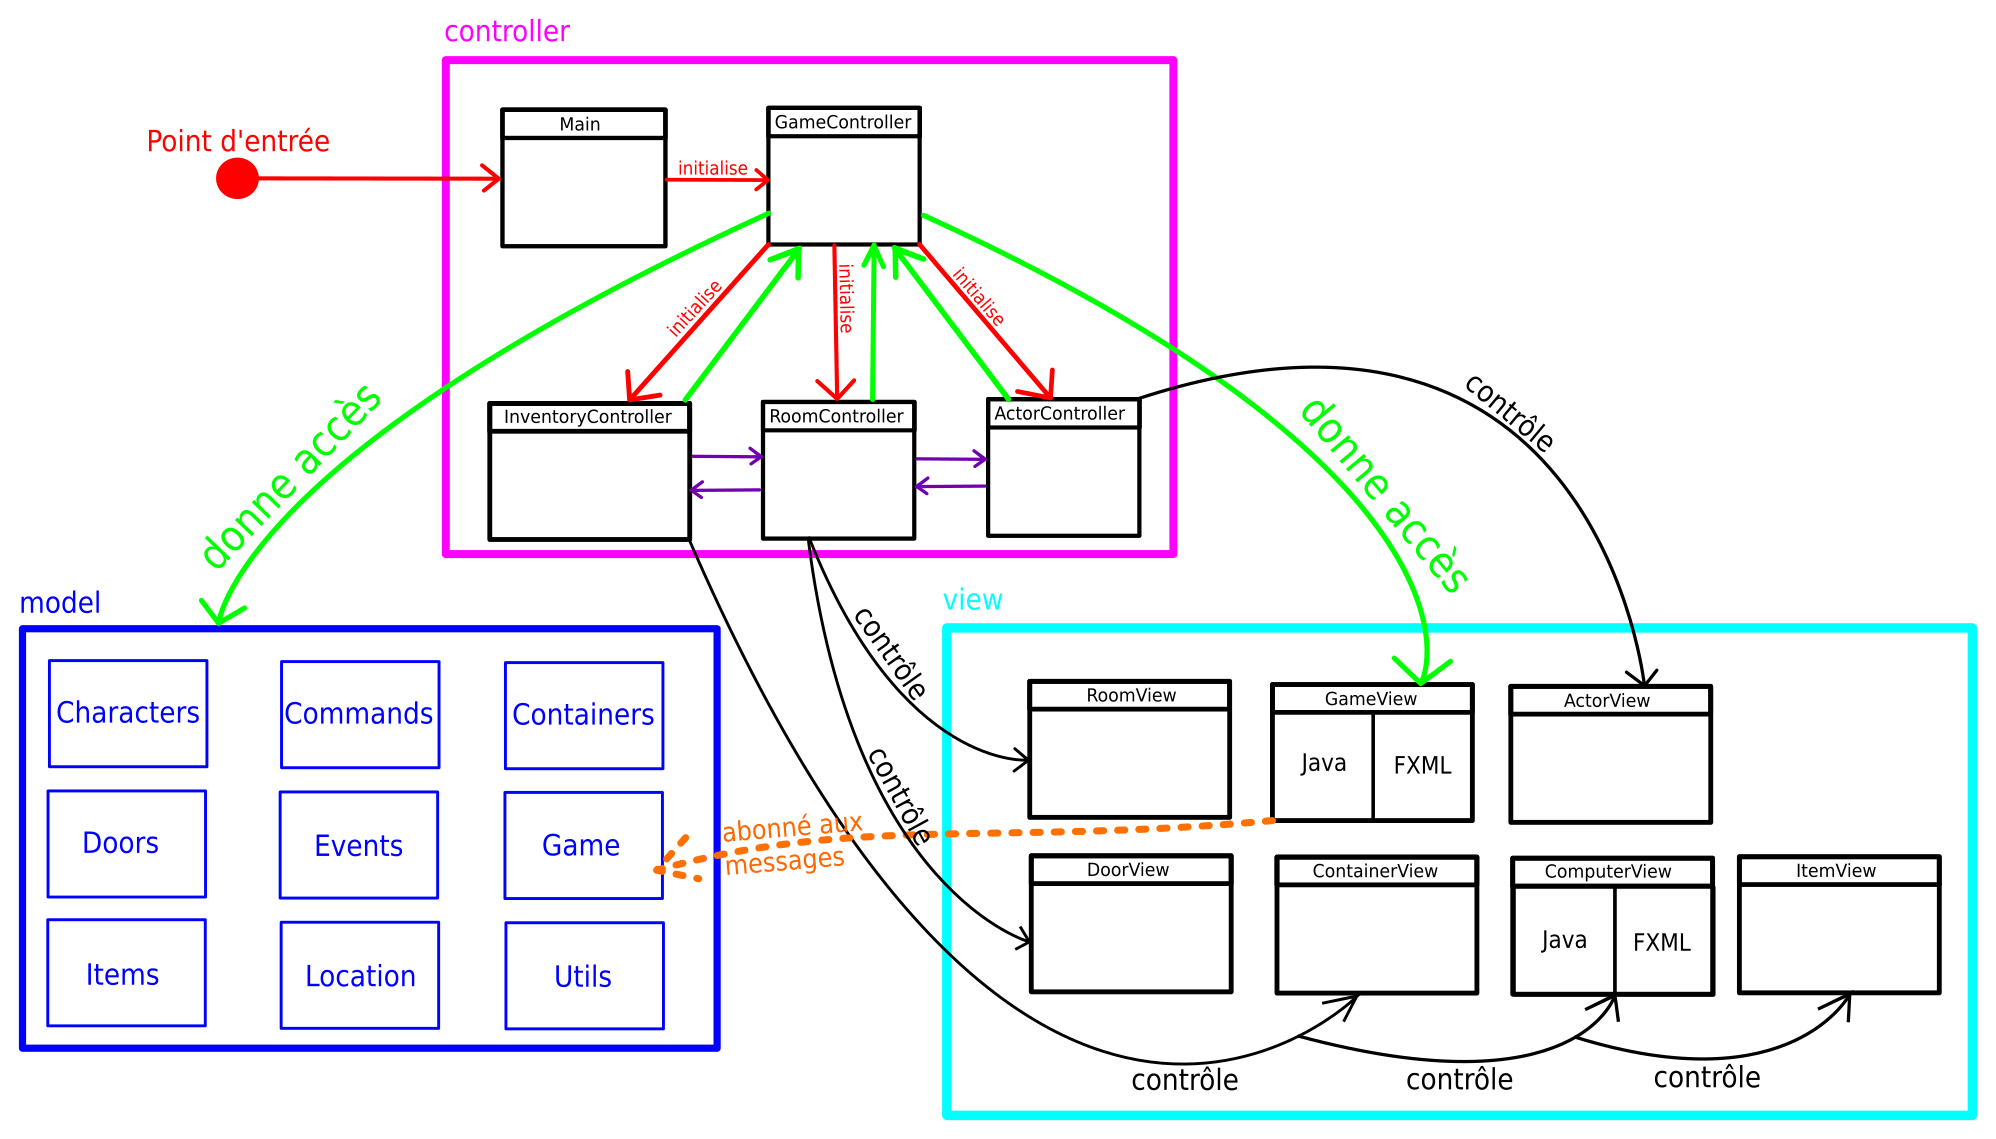
\includegraphics[scale=0.31]{images/structuration.png}
\end{center}

Le jeu se lance avec le \textit{Main} du package \textit{controller}. Ce \textit{Main} initialise le contrôleur général du jeu, appelé \textit{GameController}. Ce contrôleur lui-même lance trois autres contrôleurs spécialisés: le \textit{ActorController}, le \textit{InventoryController} et le \textit{RoomController}.\\

Le but du \textit{GameController} est d'initialiser les gestionnaires d'événements globaux du jeu (manuel d'aide et fin de la partie) et d'offrir une porte d'accès au modèle et à la vue du jeu pour les trois autres contrôleurs plus spécialisés.\\

Aussi, les trois autres contrôleurs ont tous la main sur la vue du jeu (\textit{GameView}) et sur d'autres éléments visuels dont ils sont spécialistes (comme la vue des pièces et des portes - respectivement \textit{RoomView} et \textit{DoorView} - pour le \textit{RoomController})\\

Enfin, ces trois contrôleurs peuvent avoir besoin de communiquer entre eux (flèches violettes sur le schéma). Ceci est le cas, par exemple, pour les fonctions \textit{drop()} et \textit{take()} de l'\textit{InventoryController} qui doivent nécessairement connaître la pièce dans laquelle il doivent ajouter ou retirer un élément visuel.\\

Quand ils communiquent ils le font toujours en passant par le \textit{GameController} afin d'avoir les données les plus à jour du modèle et de la vue.\\

L'objectif de cette structuration était de recréer de mini modèles MVC au sein d'un modèle MVC plus général. Cette structuration devait permettre d'éviter un contrôleur de jeu trop imposant et d'améliorer la lisibilité du code.\\

Pour terminer, nous noterons l'abonnement de la vue du jeu (\textit{GameView}) aux messages du jeu par le biais d'une interface présente dans le package \textit{Game} du modèle qui envoie les chaînes de caractère du jeu au \textit{MessageListener} enregistré. Ceci nous permettait de continuer de tester le modèle dans la commande (pour y trouver d'éventuels bugs) tout en ne changeant rien au fonctionnement général du jeu.
\newpage


% Section:
\section{Notre démarche dans la construction de cette application}
\medskip

Nous avons commencé le développement dès le lancement du projet le 20 Mars. Ayant un modèle que nous avions beaucoup testé le semestre précédent et qui ne comportait pas de bugs à notre connaissance, nous avons débuté sur le développement de la vue générale du jeu. Nous avons choisi FXML car nous pensions que c'était l'outil le plus simple pour gérer la création d'une vue aussi complexe, mais aussi parce que ce choix répondait au cahier des charges.\\

Nous avons ensuite longuement hésité sur la marche à suivre. Nous pensions que le contrôleur associé au document FXML était un "véritable" contrôleur. Aussi nous avions commencé à diviser la vue en 6 FXML différents (un pour la carte du jeu, un autre pour le panneau des acteurs, etc.)\\

En fin de compte il nous a paru plus simple de concevoir le contrôleur associé au FXML comme un moyen d'accéder dans Java aux éléments de la vue FXML. Il s'agissait donc moins d'un contrôleur et bien plus de la "partie Java" de la vue. Nous avons adopté ce point de vue suite à un entretien avec M. Bergey et nous espérons ne pas l'avoir mal interprété.\\


\paragraph{Répartition du travail\\}
Suite à ce travail de conception en collectif nous nous sommes répartis le travail entre nous:
\begin{itemize}
	\item Florian devait réaliser le chargement automatique des pièces (afin d'éviter de coder en dur les vues des 30 pièces du jeu final). Il devait également réaliser la fonction de zoom sur les pièces, les translations avec les sliders et le \textit{binding} du label (cf. élément \textbf{(2)} de l'UI présentée ci-dessus).
	\item Alexis Louail et Vincent Tourenne devaient s'occuper des interactions du joueur avec les aliens et lui-même et ils devaient également s'occuper de l'implantation en GUI de la fonction de sauvegarde et de chargement du jeu.
	\item L'implantation de l'UI de l'inventaire devait être réalisé collectivement à la fin de l'implantation des points évoqués. Cette implantation comprenait les fonctions de prise d'un objet sur le sol, d'affichage de la description des objets et de \textit{give()}, \textit{use()}, \textit{drop()}.\\
\end{itemize}

Cependant, certaines difficultés dont nous faisons la liste ci-après, nous ont amené à revoir cette répartition:
\begin{itemize}
	\item Florian a implanté ses fonctionnalités et celles de l'inventaire
	\item Alexis Louail et Vincent Tourenne ont implanté leur part\\
\end{itemize}
 
\paragraph{Obstacles et difficultés du développement\\}

Durant le développement de ce projet nous avons dû faire face à de nombreuses difficultés:
\begin{itemize}
	\item Les examens de fin d'année et les autres projets
	\item Un début de stage en 35h dès le 12 Avril pour Florian Legendre
	\item Des difficultés personnelles pour Florian Legendre (deuil de son chien)
	\item Des déplacements réguliers ainsi que des difficultés personnelles et matérielles pour Alexis Louail
	\item Des difficultés liées au partage du code sur l'IDE Intellij et aux différentes versions de Java/JavaFx avec Git (fichiers de configuration .idea/)
	\item Nos incompréhensions et fausses routes propres au travail d'un étudiant\\
\end{itemize}

\paragraph{Outils utilisés pour le développent et la gestion de ce projet\\}
L'objectif dans le choix de ces outils était de nous permettre de travailler le plus efficacement possible. Aussi nous avons choisi:
\begin{enumerate}
	\item De versionner notre code sur Git
	\item De nous le partager via un dépôt privé GitHub
	\item De communiquer régulièrement et en temps réel par des salons vocaux ou par messages sur Discord
	\item De nous répartir les bugs détectés via la fonctionnalité des tickets de GitHub
\end{enumerate}


% Section:
\section{Résolution des problèmes de conception}
Au cours du développement de cette application nous avons dû résoudre un nombre important de problèmes de conception. Certains d'entre eux ont déjà été détaillé ci-dessus et donc nous ne faisons que les mentionner ici:

\begin{itemize}
	\item Conception du modèle (semestre précédent)
	\item Adaptation du modèle (positions relatives des objets/acteurs/portes du modèle et abonnements aux messages du jeu)
	\item Structuration globale de l'architecture de l'application en nous basant sur l'architecture MVC tout en essayant d'avoir un code le plus modulaire possible (éviter d'avoir un seul gros contrôleur et plusieurs sous-contrôleurs spécialisés dont les méthodes sont des briques à utilisables pour construire des méthodes plus complexes)\\
\end{itemize}

Parmi les autres problèmes de conception les plus notables que nous avons eu à résoudre et que nous n'avons pas eu le temps encore d'expliquer il y a:

\begin{enumerate}
	\item Le chargement automatique des pièces
	\item La gestion de l'utilisation des objets
	\item La gestion du don d'objet
	\item La gestion de l'ordinateur du jeu
\end{enumerate}

\paragraph{Chargement automatique des pièces\\}
\noindent
\begin{lstlisting}[style=Java, caption={Méthode de mise à jour de la vue des pièces extraite du \textit{RoomController}}]
    public void updateRoomView(int nbCol, int nbLignes) {
        //On récupère le modèle:
        currentRoomModel = gameController.getPlayerModel().getRoom();

        //On met à jour la vue:
        gameController.getGameView().getMapPane().getChildren().remove(currentRoomView);
        currentRoomView = new RoomView(nbCol, nbLignes);
        gameController.getGameView().getRoomLabel().setText("Room " + currentRoomModel.getID());
        loadDoors();
        loadItems();
        loadPlayer();
        loadNPCs();
        loadHandlers();
        gameController.getGameView().getMapPane().getChildren().add(currentRoomView);

        //On signale à l'inventaire de mettre à jour la taille du tableau 
        //de gestionnaires d'événements utilisé pour la gestion de la
        //fonction use() des objets (quand on clique gauche sur un objet):
        gameController.getInventoryController().resetUseItemHandlersArray(nbCol, nbLignes);

        //"Éteint" l'ordinateur si le joueur quitte la pièce sans appuyer 
        //sur le bouton 'quitter':
        gameController.getActorController().resetActorPanel();

        //À chaque nouvelle pièce chargée on vérifie si le jeu est terminé:
        gameController.isGameOver();
    }
\end{lstlisting}
\newpage
On peut remarquer plusieurs problèmes à cette conception du chargement automatique:

\begin{itemize}
	\item La vue n'est pas vraiment mise à jour: elle est détruite par l'initialisation d'une toute nouvelle vue
	\item Certaines méthodes normalement du ressort de l'\textit{InventoryController} ou encore de l'\textit{ActorController} ou \textit{GameController} sont laissées à la charge du \textit{RoomController} dans cette méthode de mise à jour de la vue. Bien qu'il s'agissait de solutions 'simples' pour résoudre certains problème, nous avons conscience que nous ne pouvons pas résoudre tous les problèmes du jeu en réinitialisant tout à chaque changement de pièce.
\end{itemize}

\paragraph{Gestion de l'utilisation des objets\\}

Pour la gestion de l'utilisation des objets, deux options ont été considérées:
\begin{enumerate}
	\item Un bouton \textit{Use} présent aux côtés du bouton \textit{Give}, \textit{Drop} et \textit{Look}. Quand le joueur sélectionne un des \textit{ToggleButton} de l'inventaire, le \textit{string} du label de ce dernier est stocké dans un tableau. Le joueur aurait ensuite cliqué sur un élément visuel de la pièce ce qui aurait ajouté un second \textit{string} dans le tableau. Lorsque le joueur aurait ensuite cliqué sur le bouton \textit{Use}, ce bouton aurait appelé la fonction \textit{use()} du modèle en cherchant les éléments du modèle associés aux \textit{strings} stockés dans le tableau
	\item Nous n'utilisons pas de bouton \textit{Use}. Lorsque le joueur sélectionne un des \textit{ToggleButton} de l'inventaire, des gestionnaires d'événements sont attachés à tous les éléments visuels présents dans la pièce. Ces gestionnaires d'événements appellent la fonction \textit{use()} du modèle avec le \textit{string} de l'objet sélectionné en paramètre. Afin de gérer ces gestionnaires d'événements temporaires nous avons utilisé un tableau nommé \textit{fireHandlers} qu'on nettoyait dès que l'objet était déselectionné ou utilisé ou que le joueur changeait de pièce\\
\end{enumerate}

La dernière solution, plus complexe, a été choisie car elle nous semblait plus ergonomique et que le défi nous semblait intéressant. Cependant, elle a aussi introduit de la complexité dans notre code et une gestion d'un tableau que l'on retrouve notamment dans la méthode de mise à jour de la vue des pièces présentées ci-dessus.
\begin{center}
	\begin{figure}[h!]
	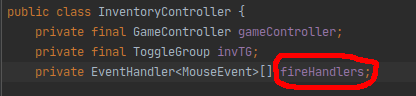
\includegraphics[scale=1]{images/fireHandlers.png}
	\caption{Le tableau \textit{fireHandlers} permettant de gérer les gestionnaires d'événements temporaires}
	\end{figure}
\end{center}

\paragraph{Gestion du don d'objet\\}

La gestion du don d'objet utilise deux informations:
\begin{enumerate}
	\item L'acteur sélectionné (cf. élément \textbf{(6)} de l'UI présentée au début de ce rapport)
	\item L'objet sélectionné (le \textit{ToggleButton} dans le panneau de l'inventaire, élément \textbf{(12)} de l'UI)
\end{enumerate}

L'étiquette du personnage est récupéré dans la vue de l'acteur sélectionné, l'étiquette de l'objet dans le \textit{ToggleButton} sélectionné de l'inventaire. Un gestionnaire d'événement est alors associé au bouton \textit{Give} qui fait appel à la méthode \textit{give()} du modèle avec ces deux informations.\\

Aussi notre solution ressemble beaucoup à la première solution envisagée pour l'utilisation des objets, le tableau de stockage des étiquettes en moins car n'étant pas nécessaire à la résolution de ce problème.
\newpage

\paragraph{Gestion de l'ordinateur du jeu\\}
Enfin, notre jeu présentait un élément spécial: un ordinateur. Dans le modèle, cet ordinateur se comportait comme un terminal de commande dans le terminal de commande. L'ordinateur contient des fichiers que le joueur peut consulter ou emporter des copies et certains de ses "programmes" permettent de déclencher des événements dans le jeu (comme l'ouverture de la porte dans la pièce 23)\\

Étant donné que dans le modèle la "vue" choisie était celle d'un terminal dans le terminal, il nous a paru naturel de lui donner une traduction graphique "d'ordinateur dans l'ordinateur" pour cette application.\\

Aussi l'ordinateur a son propre mini-MVC. Lorsque l'ordinateur est utilisé par le joueur, le contrôleur de ce mini-MVC est appelé et remplace le panneau de l'acteur comme illustré dans l'image ci-dessous:

\begin{center}
	\begin{figure}[h!]
	\advance\leftskip-0.6cm
	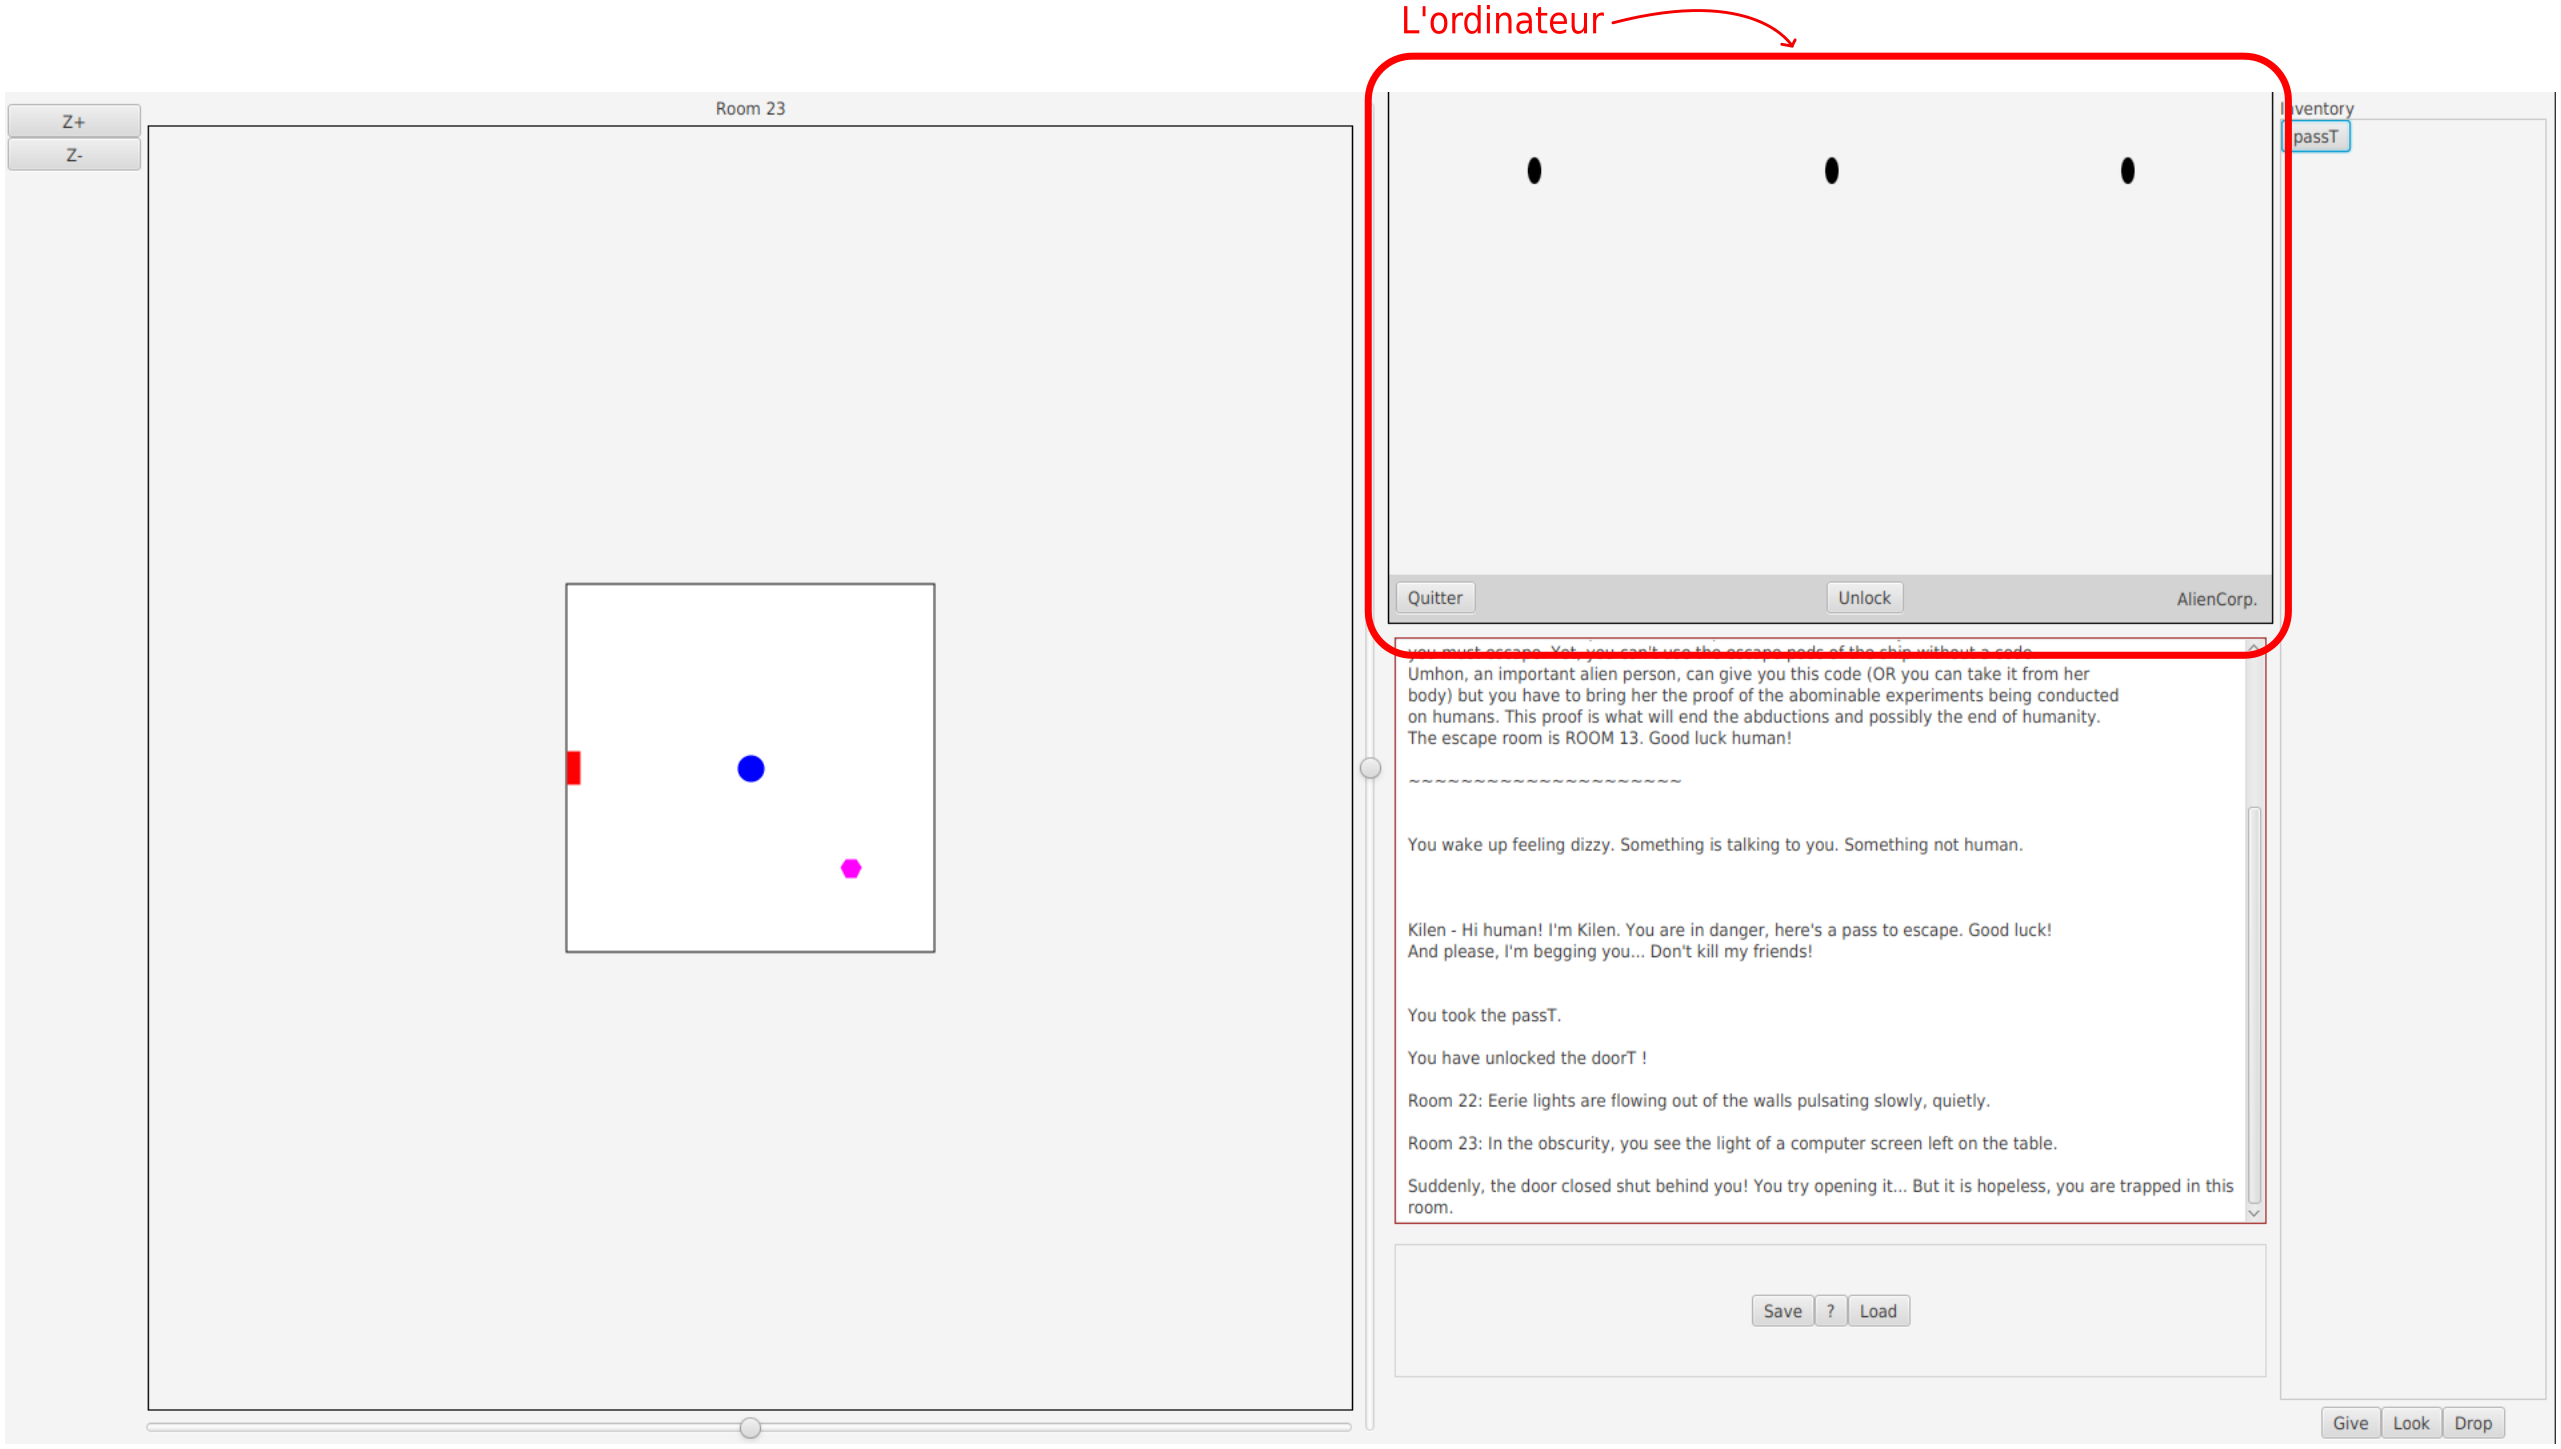
\includegraphics[scale=0.25]{images/ordinateur.png}
	\caption{Illustration de la vue de l'ordinateur dans le jeu, les fichiers réutilisent la vue des items du jeu et sont représentés par des ellipses noires}
	\end{figure}
\end{center}

La solution de la fenêtre popup a été considérée et aurait permise de simplifier la gestion de la fermeture de l'ordinateur lorsque le joueur quitte une pièce sans avoir cliqué sur le bouton 'quitter'. Cette gestion est actuellement assuré par la méthode \textit{updateRoomView} du \textit{RoomController} présenté précédemment.\\

Cependant, nous tenions à éviter l'utilisation des fenêtres popups car nous jugions qu'elles cassaient un peu le rythme du jeu.\\

La gestion complète de l'ordinateur est inachevée et fait partie des axes d'amélioration et des possibilités d'extension de l'application dont nous voulons maintenant faire l'état dans la section suivante de ce rapport.

\newpage

% Section:
\section{Analyse des possibilités d’extension de l’application}
\medskip

\paragraph{Les axes d'amélioration\\}
Le présent rendu est un travail inachevé. Les premiers points d'achèvement que nous souhaiterions aborder sont:

\begin{itemize}
	\item Davantage clarifier la responsabilité de chaque contrôleur
	\item Renforcer la modularité du code
	\item Éliminer les quelques données laissées en dur dans le code
	\item Optimiser certaines méthodes en évitant de mettre à jour toute la pièce mais seulement quelques éléments de la pièce par le biais de méthodes \textit{load()} et de méthodes \textit{unload()}
	\item Revoir le système de conversion des objets du modèle en leurs vues\\ respectives\\
\end{itemize}

Dans l'état actuel des choses nous pensons pouvoir produire le jeu final que nous espérions. En effet:

\begin{itemize}
	\item Le chargement des pièces est automatique aussi l'ajout d'une pièce dans le modèle provoque l'ajout d'une pièce dans la vue
	\item La vue est abonnée aux messages du jeu aussi l'ajout de dialogues dans le jeu sont automatiquement restranscrits dans la vue
	\item 100\% des fonctions du modèles sont implantées et ont leurs équivalents dans la présente interface\\
\end{itemize}

Mais développer l'application finale sans retravailler les points énoncées ci-dessus nous amènerait probablement à produire un code lourd (notamment si on ajoute de nouveaux objets) dans son exécution et pas très lisible.\\

De plus, il faudrait renforcer le nombre de cas possibles: il est prévu dans le modèle des pièces qui ne comportent pas nécessairement 4 portes. Pour l'ordinateur nous n'avons pas prévu de comportement dans le cas où le nombre de fichiers excéderaient la capacité de la vue, etc.\\

\paragraph{Les fonctionnalités futures envisagées\\}
En dernier lieu, quand tous ces points trouveront leurs implantations dans l'applications, nous pensions améliorer le visuel du jeu en utilisant de nouveaux \textit{assets}, en utilisant des services qui modifieraient la couleur des pièces selon un gradient qui donnerait un effet de pulsation lumineuses au vaisseau, peut-être même en préchargeant les pièces voisines pour aider le joueur à s'orienter, etc.\\

D'autres éléments d'ergonomie peuvent être reconsidérés: le bouton \textit{Give} n'est pas très pratique à utiliser, les boutons de ZOOM+ et de ZOOM- pourraient être remplacés par un \textit{binding} sur la molette de la souris du joueur, les sliders pourraient être remplacés par un drag \& drop de la pièce avec la souris, etc.

\newpage

% Section:
\section{Erreurs détectées et commentaires}

Au cours du développement nous avons détecté de nombreuses erreurs que nous avons corrigé en nous répartissant le travail par le biais de tickets:

\begin{center}
	\begin{figure}[h!]
	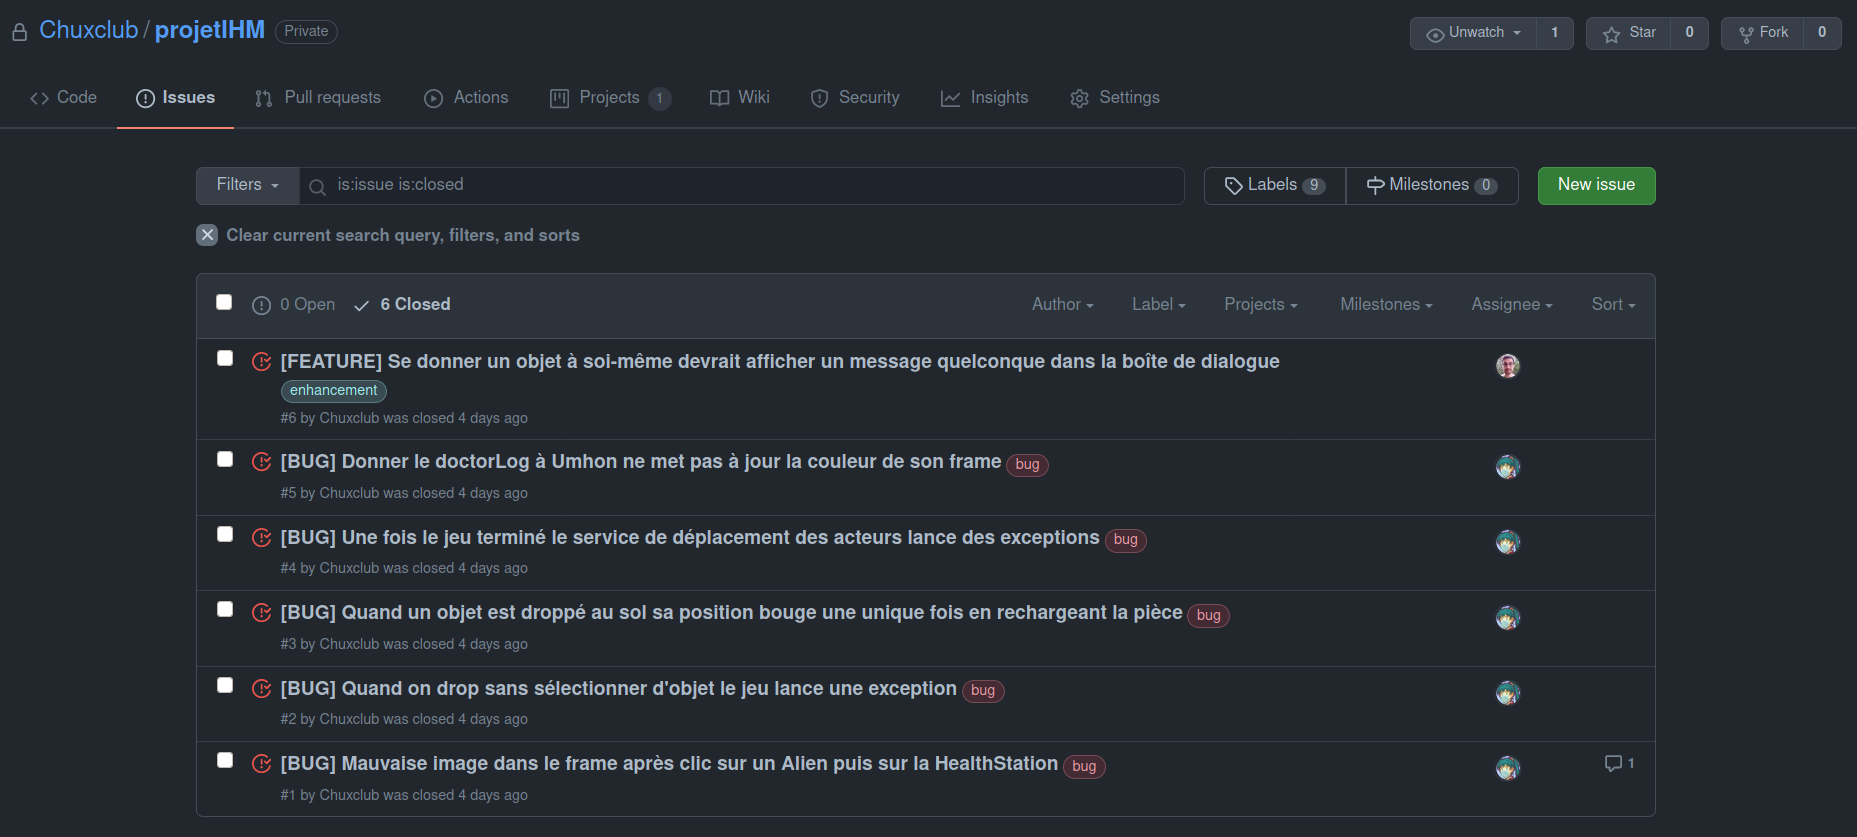
\includegraphics[scale=0.25]{images/tickets.png}
	\caption{Des tickets de bug sous GitHub}
	\end{figure}
\end{center}

Ces erreurs étaient détectées soit au cours de nos propres tests de l'application, soit en laissant l'application aux mains de nos proches. Ces-derniers sont en remerciement dans la fenêtre popup de fin de partie.\\

Au moment du rendu de cette application nous n'avons pas détecté de nouveaux bugs.


\newpage

\end{document}